% The two-object poset 0 ≤ 1 as a category (identities shown).
% Source: book/tex/cats/functors.tex (§ Natural transformations).
\documentclass[border=2mm]{standalone}
\usepackage{tikz}
\usetikzlibrary{arrows.meta}
\newcommand{\id}{\mathrm{id}}
\begin{document}
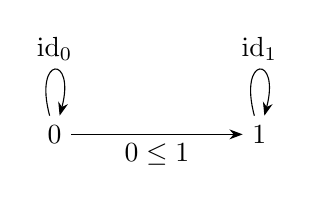
\begin{tikzpicture}[>=Stealth, every loop/.style={min distance=8mm, looseness=14}]
  \node (0) at (0,0) {$0$};
  \node (1) at (2.6,0) {$1$};
  \draw[->] (0)--(1) node[midway,below]{$0\le 1$};
  \draw[->] (0) to[loop above] node[above]{$\id_0$} (0);
  \draw[->] (1) to[loop above] node[above]{$\id_1$} (1);
\end{tikzpicture}
\end{document}
